\section{Journey planning}
\label{sec:etas-journey-planning}



So far we have been concerned with the arrival time for a bus at a single stop with no consideration of the passenger's commute as a whole. The most straightforward journey consists of a single route choice, so the only decision is which trip to catch; a slightly more complex journey may offer two alternative routes (\cref{sec:journey_simple}) between which the passenger may choose. Finally, there may be no single route which goes from the passenger's start location to their destination, in which case a transfer between two (or more) different routes, or \emph{legs}, is necessary (\cref{sec:journey_transfer}).


Dynamic routing---the selection of candidate trips and real-time assessment of which is \emph{optimal}---is in itself a difficult problem to solve \citep{Hame_2013a,Hame_2013b,Zheng_2016}. There also exist implementations which can take a probabilistic model of arrival time (such as we can obtain by \glspl{cdf}) as input to determine the optimal route (including the selection of candidate routes), such as proposed by \citet{Berczi_2017}. Therefore, for this section we only consider choosing between pre-selected candidate journey options using the arrival time \glspl{cdf} obtained using our \pf{} model. These are compared to the results one might obtain using the currently deployed schedule-delay predictions, which only provide a binary (`Yes' or `No') prediction.


\begin{knitrout}\small
\definecolor{shadecolor}{rgb}{0.969, 0.969, 0.969}\color{fgcolor}\begin{figure}

{\centering 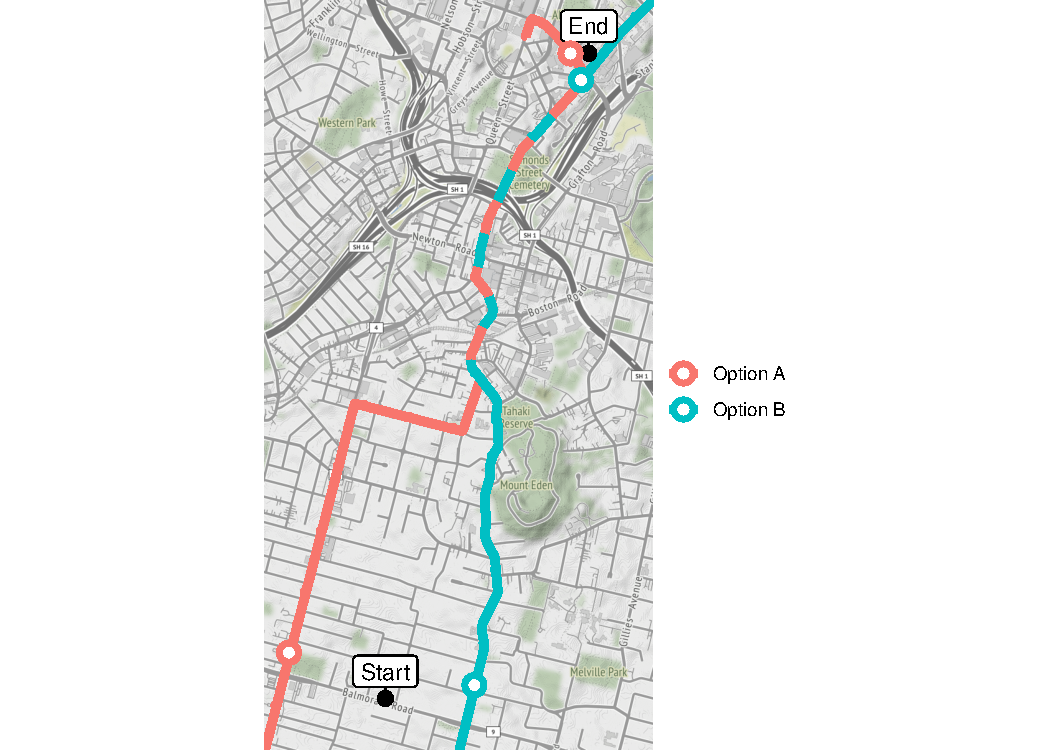
\includegraphics[width=\textwidth]{figure/eta_journey_arrival_prep-1} 

}

\caption[Route options]{Route options}\label{fig:eta_journey_arrival_prep}
\end{figure}


\end{knitrout}

\subsection{Choosing between two alternative routes}
\label{sec:journey_simple}

In this scenario, a passenger lives within walking distance of two major roads, along which various routes travel into the central city, as displayed in \cref{fig:eta_journey_arrival_prep}. The passenger needs to decide which route option to take before leaving home and let's say they have an appointment in town at  2:00~pm. At  1:20~pm, they consult the real-time app on their phone before deciding whether to walk to route option A or B. Factors that could influence their decision include:
\begin{itemize}
\item how long they will have to wait for the next bus;
\item the probability that they will arrive in time for the next bus, and how long until the bus after it;
\item the probability of arriving at their destination on-time, and how early they will be; and
\item the overall length of the journey.
\end{itemize}
We can provide information relating to these questions using the \glspl{cdf} of arrival time at the start and end stops. Walking times at either end of the journey can also be accounted for.


\begin{knitrout}\small
\definecolor{shadecolor}{rgb}{0.969, 0.969, 0.969}\color{fgcolor}\begin{figure}

{\centering 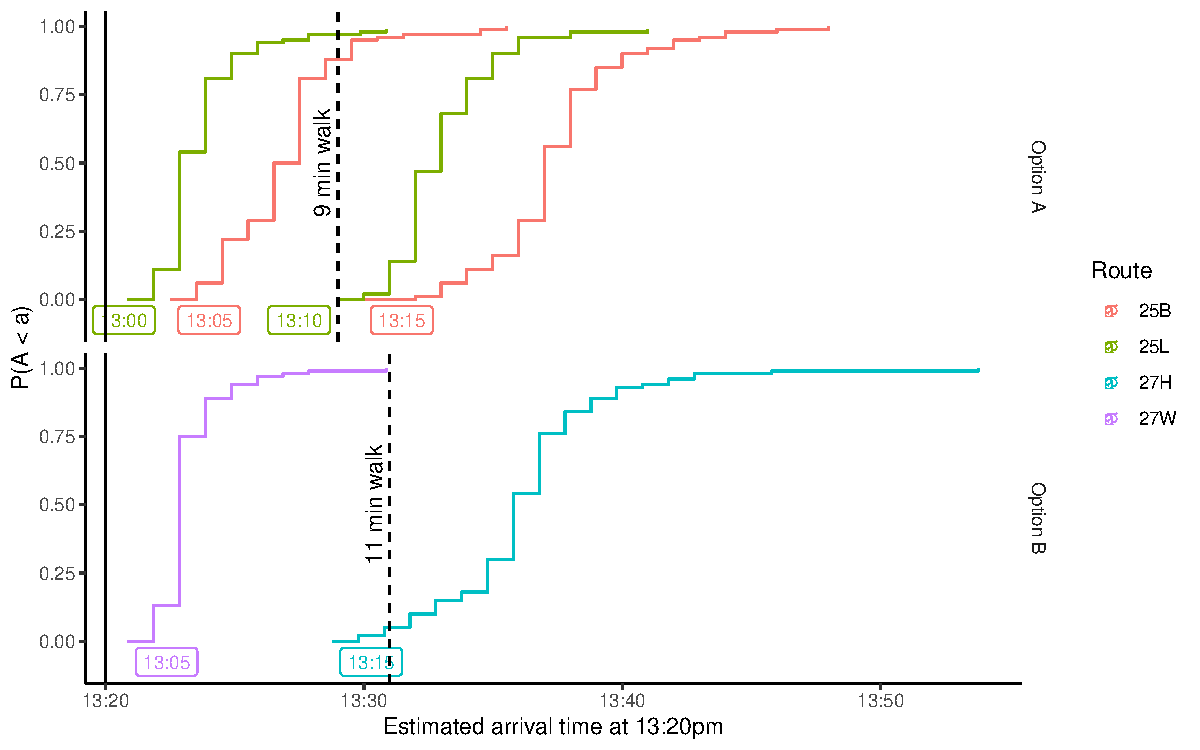
\includegraphics[width=\textwidth]{figure/eta_journey_arrival-1} 

}

\caption[ETA predictions for two route options]{ETA predictions for two route options. The coloured curves represent the CDF of arrival time for individual trips made at 7~am. The vertical black lines indicate the estimated walking time (according to Google Maps) from the Start location to each stop.}\label{fig:eta_journey_arrival}
\end{figure}


\end{knitrout}



\Cref{fig:eta_journey_arrival} displays the \glspl{cdf} of all active trips\footnote{Our application currently only estimates arrival times for active trips.} along the two route options at  1:20~pm when the passenger is about to leave home (solid line), with dashed lines representing the passenger's arrival time at the stops (accounting for walking time). Below each \gls{cdf}, which are coloured by route number, is a label indicating the trip's start time, which is the simplest method of identifying trips. For option A, there appears to be a minimal chance of catching the 1:05~pm 25B, but a good chance of catching the 1:10~pm 25L, with the additional safety of another 25B not long after. As for option B, there is a slightly smaller chance of catching the 1:15~pm 27H, but if missed, it is unclear how long the wait for the next but will be.


\begin{knitrout}\small
\definecolor{shadecolor}{rgb}{0.969, 0.969, 0.969}\color{fgcolor}\begin{figure}

{\centering 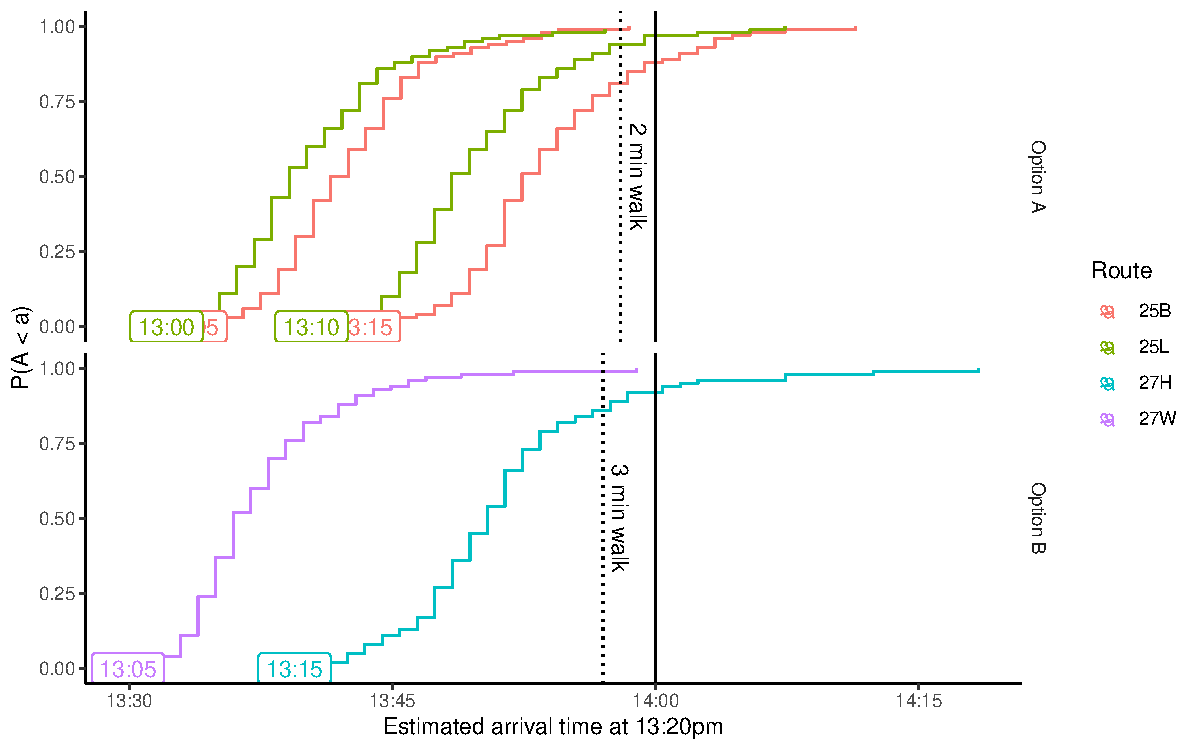
\includegraphics[width=\textwidth]{figure/eta_journey_arriveby-1} 

}

\caption[ETA predictions for two route options]{ETA predictions for two route options. The coloured curves represent the CDF of arrival time for individual trips made at 7~am. The vertical black lines indicate the estimated walking time (according to Google Maps) from the Start location to each stop.}\label{fig:eta_journey_arriveby}
\end{figure}


\end{knitrout}

Based on the arrival results alone, I would choose to walk to option A as it has a good chance of a short wait time; however, the passenger also needs to consider their appointment at 9~am. \Cref{fig:eta_journey_arriveby} provides \glspl{cdf} of each trip's arrival time at the final stop, as well as vertical lines representing the appointment time (solid) and necessary arrival time to allow for walking time (dotted). None of the trips show definitive signs of being late, although the passenger would likely hope to catch the 1:10~pm 25L to maximise their chances of arriving on-time.


\begin{knitrout}\small
\definecolor{shadecolor}{rgb}{0.969, 0.969, 0.969}\color{fgcolor}\begin{table}

\caption{\label{tab:eta_journey_results}Journey planning.}
\centering
\fontsize{8}{10}\selectfont
\begin{tabular}[t]{lllrrllll}
\toprule
\multicolumn{1}{c}{} & \multicolumn{1}{c}{} & \multicolumn{1}{c}{} & \multicolumn{2}{c}{Particle filter} & \multicolumn{2}{c}{GTFS} & \multicolumn{2}{c}{Outcome} \\
\cmidrule(l{3pt}r{3pt}){4-5} \cmidrule(l{3pt}r{3pt}){6-7} \cmidrule(l{3pt}r{3pt}){8-9}
Option & Route & Trip & $P_\text{catch}$ & $P_\text{arrive}$ & Catch & Arrive & Caught & Arrived\\
\midrule
A & 25L & 13:00 & 0.02 & 0.99 & N & Y & N & Y\\
 & 25B & 13:05 & 0.05 & 0.99 & N & Y & N & Y\\
 & 25L & 13:10 & 0.98 & 0.94 & Y & Y & Y & Y\\
 & 25B & 13:15 & 1.00 & 0.81 & Y & N & Y & Y\\
\midrule
B & 27W & 13:05 & 0.00 & 0.99 & N & Y & N & Y\\
 & 27H & 13:15 & 0.90 & 0.86 & Y & Y & Y & Y\\
\bottomrule
\end{tabular}
\end{table}


\end{knitrout}


The \glspl{cdf} allow easy calculation of the predicted probability of success in each scenario, displayed in \cref{tab:eta_journey_results}. Additionally, the binary (`Yes' or `No') predictions made using the schedule-delay method are displayed for comparison, as well as the eventual outcome. That is, would the passenger have caught the bus and did it arrive on time? All of the predictions based on the \pf{} arrival time \glspl{cdf} are valid: small probabilities correspond to an outcome of `No' and large probabilities ($>0.8$) to `Yes'. There was a discrepancy for the 1:15~pm 25B, which arrived at the destination on time: the schedule-delay incorrectly predicted `No', while our method predicted an 81\% chance of success.


\begin{knitrout}\small
\definecolor{shadecolor}{rgb}{0.969, 0.969, 0.969}\color{fgcolor}\begin{figure}

{\centering 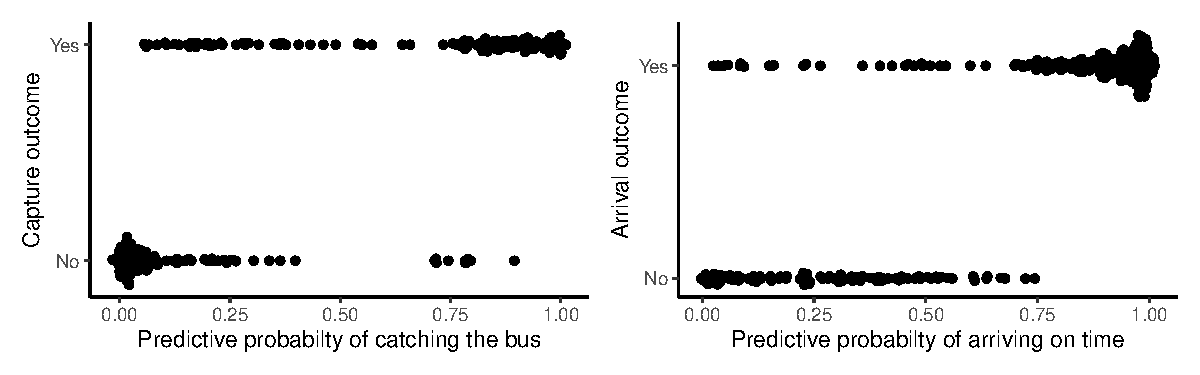
\includegraphics[width=\textwidth]{figure/eta_journey_results_avg-1} 

}

\caption[Results of performing the same journey planning prediction with different starting times (from  9:00~am to  3:00~pm), using the same start and end locations]{Results of performing the same journey planning prediction with different starting times (from  9:00~am to  3:00~pm), using the same start and end locations. Observations are whether or not the passenger would have arrived at the stop before the bus, jittered to better see each observation. Predictive probabilities of 0 and 1 that were correctly estimated have been removed.}\label{fig:eta_journey_results_avg}
\end{figure}

\begin{table}

\caption{\label{tab:eta_journey_results_avg}GTFS prediction results over all journeys, with the displayed values representing the proportion of outcomes in each cell (rows are conditioned by the GTFS prediction of Yes or No. }
\centering
\fontsize{8}{10}\selectfont
\begin{tabular}[t]{llllll}
\toprule
\multicolumn{1}{c}{} & \multicolumn{5}{c}{Observed outcome} \\
\cmidrule(l{3pt}r{3pt}){2-6}
\multicolumn{1}{c}{ } & \multicolumn{2}{c}{Catch bus} & \multicolumn{1}{c}{} & \multicolumn{2}{c}{Arrive on time} \\
\cmidrule(l{3pt}r{3pt}){2-3} \cmidrule(l{3pt}r{3pt}){5-6}
GTS Prediction & No & Yes &  & No & Yes\\
\midrule
No & 0.98 & 0.02 &  & 0.78 & 0.22\\
Yes & 0.09 & 0.91 &  & 0.00 & 1.00\\
\bottomrule
\end{tabular}
\end{table}


\end{knitrout}

The results in \cref{fig:eta_journey_arrival,fig:eta_journey_arriveby} and \cref{tab:eta_journey_results} are based on \emph{one single forecast} made at  1:20~pm. To evaluate the overall performance of our prediction method, we repeated the process described above in 5~minute intervals over the off-peak period from  9:00~am to  3:00~pm. For the appointment time, we used 30~minute intervals allowing for 15--45 minutes for the journey: leaving between 9:15~am and 9:45~am had a targetted arrival time of 8:00~am; 9:45~am--10:15~am targetted 8:30~am; and so on. The probabilities of catching the bus and arriving on time were calculated for each case. \Cref{fig:eta_journey_results_avg}, graphs the distribution of predicted probabilities for each of the two outcomes, for both catching the bus (left) and arriving on time (right). For most of the buses that arrived before the passenger, our method predicted capture probability below 50\%, though more buses which arrived after the passenger also had capture probabilities below 50\%. As for the arrival outcome, the maximum probability of arriving on time for buses which did not was 75\%, whereas a few buses which did arrive on time had small (< 50\%) probabilities of doing so.


For comparison, \cref{tab:eta_journey_results_avg} presents a two-way contingency table for the binary schedule-delay predictions, with the predicted outcomes in rows. Where the schedule-delay predicted that the bus would arrive after the passenger, it was correct 91\% of the time. When it predicted the bus would arrive first, it had a 98\% success rate. As for the arrival, in all cases that the schedule-delay predicted the bus would arrive on time, it was correct, versus only 78\% when it predicted the bus would be late. Overall, the schedule-delay method correctly predicted the bus capture outcome in 94\% of cases and correctly predicted the on-time arrival outcome in 89\% of cases.


In both methods, predicting bus capture is more accurate than predicting on-time arrival, which is acceptable considering the difference in forecast length: about 10~minutes for bus capture versus about 30~minutes for arrival. The schedule-delay predictions have a 1-in-10 chance of missing the bus, while our \pf{} provides a less definite prediction (such as 75\%), opening up the opportunity for passengers to make more informed decisions based on these probabilities and the importance of their constraints. In contrast, the schedule-delay method provides, at best, the predicted arrival time as a singular point estimate with no associated uncertainty, allowing only a `Yes' or `No' prediction to be made.


\subsection{Planning a multi-stage journey}
\label{sec:journey_transfer}

A more complex scenario is one in which the passenger must transfer from one route to another. Transfer journeys are common among travellers commuting from further afield, and occur when there is no single route between their origin and destination, as is demonstrated in \cref{fig:eta_journey_arrival_prep}. In this scenario, the passenger must first catch a bus along route group A\footnote{We use route groups since there are several different routes which make the same journey, as can be seen with route group B in the south-west of \cref{fig:eta_journey_arrival_prep}.} to the stop marked ``Transfer'', at which point they disembark and wait for the next bus along route group B to get to their final destination.


\begin{knitrout}\small
\definecolor{shadecolor}{rgb}{0.969, 0.969, 0.969}\color{fgcolor}\begin{figure}

{\centering 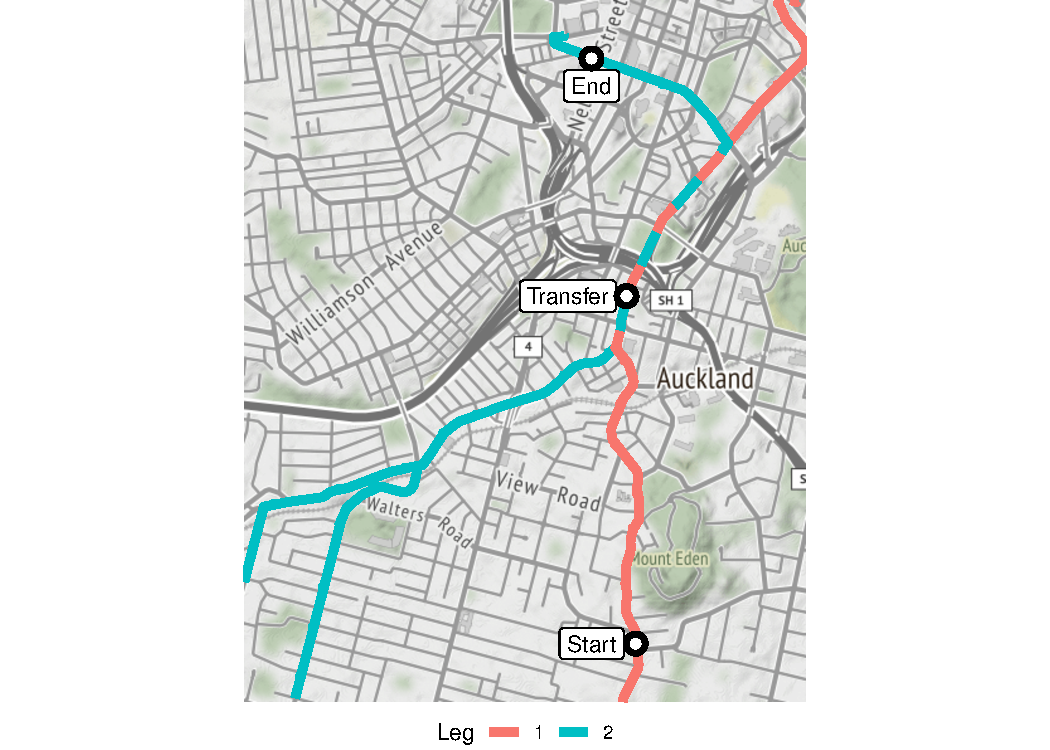
\includegraphics[width=\textwidth]{figure/eta_journey_transfer_prep-1} 

}

\caption[Transfer options]{Transfer options}\label{fig:eta_journey_transfer_prep}
\end{figure}


\end{knitrout}



\begin{knitrout}\small
\definecolor{shadecolor}{rgb}{0.969, 0.969, 0.969}\color{fgcolor}\begin{figure}

{\centering 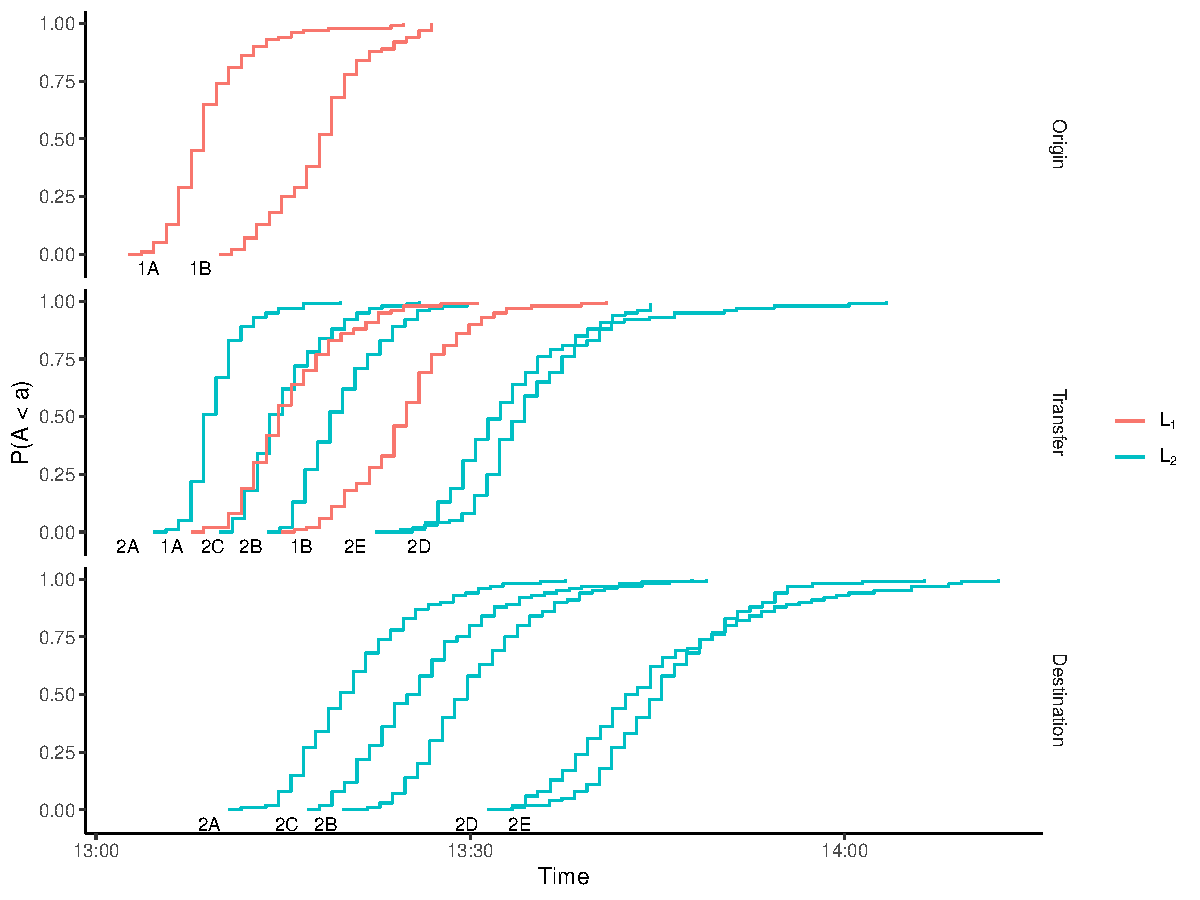
\includegraphics[width=\textwidth]{figure/eta_journey_transfer_graph-1} 

}

\caption[Arrival times]{Arrival times}\label{fig:eta_journey_transfer_graph}
\end{figure}


\end{knitrout}


Similarly to the previous example, we take one single forecast of all trip arrivals at 1~pm. Walking time has been removed to simplify the example, but could easily be included if desired. \Cref{fig:eta_journey_transfer_graph} shows, for all active trips at  1:00~pm, their arrival time \glspl{cdf} at the start and transfer stops (for the first leg) and the transfer and end stops (for the second). Additional constraints, such as arrival by a specific time, could, of course, be added; in this instance, however, we are solely interested in how well we can predict a successful transfer from A to B.


Given \glspl{cdf} for two trips arriving at a stop, the probability that a transfer can successfully be made from A to B is calculated by
\begin{equation}
\label{eq:eta_total_prob}
\begin{split}
\Pcatch =
\Pr{A < B} &= \sum_{x=1}^{\infty} \Pr{A < B\,|\,B = x}\Pr{B=x} \\
  &= \sum_{x=1}^\infty
    \Pr{A < x} \Pr{B=x} \\
  &= \sum_{x=1}^\infty
    \Pr{A < x} \left[
      \Pr{B < x + 1} - \Pr{B < x}
    \right],
\end{split}
\end{equation}
which is easily computed from the arrival time \glspl{cdf} obtained from \cref{eq:pf_pdf_arrivaltime}. \Cref{tab:eta_journey_transfer_res} displays the prediction probabilities, along with the binary predictions using the schedule-delay method and the observed outcomes.


\begin{knitrout}\small
\definecolor{shadecolor}{rgb}{0.969, 0.969, 0.969}\color{fgcolor}\begin{table}

\caption{\label{tab:eta_journey_transfer_res}Transfer probabilities}
\centering
\fontsize{8}{10}\selectfont
\begin{tabular}[t]{llrll}
\toprule
Leg 1 & Leg 2 & $\mathbb{P}_\text{transfer}$ & GTFS & Outcome\\
\midrule
1A & 2A & 0.04 & N & N\\
 & 2B & 0.71 & Y & Y\\
 & 2C & 0.32 & Y & N\\
 & 2D & 1.00 & Y & Y\\
 & 2E & 0.99 & Y & Y\\
\midrule
1B & 2A & 0.00 & N & N\\
 & 2B & 0.20 & N & N\\
 & 2C & 0.05 & N & N\\
 & 2D & 0.96 & Y & Y\\
 & 2E & 0.93 & Y & Y\\
\bottomrule
\end{tabular}
\end{table}


\end{knitrout}


The particle filter predicts transfer probabilities with reasonable accuracy: low probabilities result in negative ('No') outcomes. In contrast, the schedule-delay predictions fail to correctly predict the outcome of a transfer between 1A and 2C: it incorrectly predicted a successful transfer while the particle filter predicted only a 32\% chance of success. Here a passenger could, where applicable, base their decision on how important it is they make the transfer which might depend on frequency or other constraints. While this example is somewhat trivial (it's a short wait for the next bus), there are situations where the headway between trips is 30--60~minutes, in which case---from personal experience---watching your next bus depart just as the one you are on arrives at the station is very frustrating. However, until our application has been updated to make predictions for upcoming (and not just active) trips, we are not yet able to make predictions for such scenarios.


\begin{knitrout}\small
\definecolor{shadecolor}{rgb}{0.969, 0.969, 0.969}\color{fgcolor}\begin{figure}

{\centering 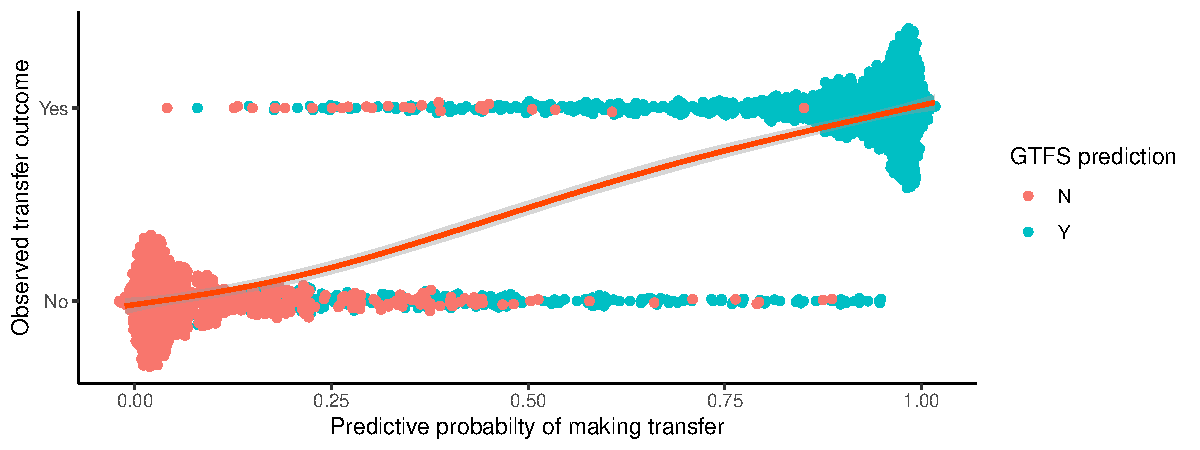
\includegraphics[width=.5\textwidth]{figure/eta_journey_transfer_many-1} 

}

\caption[Results of performing the same transfer journey planning prediction with different starting times (from  9h00 to 15h00)]{Results of performing the same transfer journey planning prediction with different starting times (from  9h00 to 15h00). Observations are whether or not the first bus would arrive at the transfer stop before the second bus, jittered to better see each observation. Additionally, predictive probabilities of 0 and 1 have been removed since, after checking, none or these were invalid and only served to distort the figure.}\label{fig:eta_journey_transfer_many}
\end{figure}

\begin{table}

\caption{\label{tab:eta_journey_transfer_many}Results of running the transfer prediction problem over the course of the day. Rows represent the predicted outcome (No, the transfer will be made, or Yes, it will) and the numbers represent the proportion of predictions with each observed outcome. The GTFS rule is binary, while the particle filter results are based on transfer probability of at least 0.5, 0.8, or 0.95 (as indicated).}
\centering
\fontsize{8}{10}\selectfont
\begin{tabular}[t]{llllllllllll}
\toprule
\multicolumn{1}{c}{} & \multicolumn{11}{c}{Outcome} \\
\cmidrule(l{3pt}r{3pt}){2-12}
\multicolumn{1}{c}{} & \multicolumn{2}{c}{GTFS} & \multicolumn{1}{c}{} & \multicolumn{2}{c}{PF (P > 0.5)} & \multicolumn{1}{c}{} & \multicolumn{2}{c}{PF (P > 0.8)} & \multicolumn{1}{c}{} & \multicolumn{2}{c}{PF (P > 0.95)} \\
\cmidrule(l{3pt}r{3pt}){2-3} \cmidrule(l{3pt}r{3pt}){5-6} \cmidrule(l{3pt}r{3pt}){8-9} \cmidrule(l{3pt}r{3pt}){11-12}
Prediction & No & Yes &  & No & Yes &  & No & Yes &  & No & Yes\\
\midrule
No & 0.97 & 0.03 &  & 0.94 & 0.06 &  & 0.85 & 0.15 &  & 0.7 & 0.3\\
Yes & 0.1 & 0.9 &  & 0.07 & 0.93 &  & 0.03 & 0.97 &  & 0 & 1\\
\bottomrule
\end{tabular}
\end{table}


\end{knitrout}



As before, the procedure was repeated in 5~minute intervals between  9:00~am and  3:00~pm, and the probabilities of transfers computed for each. \Cref{fig:eta_journey_transfer_many} shows the predicted transfer probabilities grouped by the outcome. To complement these results, \cref{tab:eta_journey_transfer_many} shows the outcomes for the schedule-delay method along with particle filter predictions using three decision rules. For the schedule-delay method, in 10\% of cases, a predicted successful connection failed versus only 7\% using the particle filter with a decision rule of $\Pcatch > 0.5$. The false-positive rate was similar for both methods, although slightly higher for our own (6\% versus 3\%). However, depending on the passenger's requirements, it is possible to reduce the false-positive rate under the particle filter by increasing the threshold.  \Cref{tab:eta_journey_transfer_many}  also shows the results using 0.8 and 0.95 as the decision rule, which results in a 3\% and 0\% false positive rate, respectively, though these result in quite a significant increase in the false-negative rate. By providing probabilities, the passenger has the option to decide what level of risk they are willing to take depending on personal constraints.


In this section, we have seen that having access to the full distribution of arrival times enables calculation of event probabilities as opposed to binary outcome predictions. Probabilities allow for more sophisticated decision making by travellers depending on their own needs, or by journey planning software and dynamic routing methods \citep{Berczi_2017}. A further advantage of using the \pf{} to estimate the \glspl{cdf} is that any improvements to the vehicle or network models will be integrated into the arrival prediction component, making future improvements simple to implement.
